\documentclass[a4paper, 12pt, titlepage]{report}

%Taal: Nederlands ("Inhoudsopgave", "Hoofdstuk",...)
\usepackage{graphicx}
\usepackage{subcaption}
\usepackage{algorithmic}
\usepackage{amsmath, amssymb, textcomp, mathtools}
\usepackage{mcode}

%Hyperlinks
\usepackage{hyperref}

%Opmaak hyperlinks
\hypersetup{colorlinks=false,	urlcolor=cyan,pdfborder=0 0 0}

%Geen nummering bij secties en hoofdstukkden
\setcounter{secnumdepth}{-1} 

%geen indents
\setlength\parindent{0pt}

\usepackage{listings}
\lstset{
language=Matlab, % choose the language of the code
%basicstyle=10pt, % the size of the fonts that are used for the code
numbers=left, % where to put the line-numbers
numberstyle=\footnotesize, % the size of the fonts that are used for the line-numbers
stepnumber=1, % the step between two line-numbers. If it's 1 each line will be numbered
numbersep=5pt, % how far the line-numbers are from the code
%backgroundcolor=\color{grey}, % choose the background color. You must add \usepackage{color}
showspaces=false, % show spaces adding particular underscores
showstringspaces=false, % underline spaces within strings
showtabs=false, % show tabs within strings adding particular underscores
frame=single, % adds a frame around the code
%tabsize=2, % sets default tabsize to 2 spaces
%captionpos=b, % sets the caption-position to bottom
breaklines=true, % sets automatic line breaking
breakatwhitespace=false, % sets if automatic breaks should only happen at whitespace
escapeinside={\%*}{*)} % if you want to add a comment within your code
}


%"Figuur" in vet
\makeatletter
\renewcommand{\fnum@figure}{\small\textbf{\figurename~\thefigure}}
\makeatother

\usepackage[dutch]{babel}
\begin{document}

\title{\textbf{Numerieke Modellering en Benadering}}
\author{De Wolf Peter\\ Vekemans Wout}

\date{\today}
\begin{titlepage}
	\maketitle
	\thispagestyle{empty}
\end{titlepage}

\newpage
\tableofcontents

\listoffigures

\newpage
\section{Benaderen met veeltermen}
In dit practicum willen we eerst enkele functies benaderen met behulp van veeltermen door interpolatie. We gebruiken hiertoe nulpunten van orthogonale veeltermen als interpolatiepunten.
\subsection{Berekenen van nulpunten van orthogonale veeltermen}
Zie bijlage \texttt{poly\_zeros.m}\\
Deze functie berekent de nulpunten van de orthogonale veeltermen gebaseerd op de waarden $\alpha_k, \beta_k$, en $\lambda_k$ uit de recursiebetrekking voor orthogonale veeltermen \eqref{recursion}. Het doet dit door een tridiagonale matrix op te stellen met elementen afgeleid van de co\"efficienten uit die recursiebetrekking. De nulpunten van de veelterm zijn dan gelijk aan de eigenwaarden van die matrix.\\
\begin{subequations} \label{recursion}
\begin{align}
\phi_0(x) = \lambda_0\; ;\; \phi_1(x) = \lambda_1(x-\alpha_1)\phi_0(x))\\
\phi_k(x) = \lambda_k(x-\alpha_k)\phi_{k-1}(x))-\beta_k\phi_{k-2}(x)
\end{align}
\end{subequations}

\subsection{Evauleren van drietermsrecursiebetrekking}
Zie bijlage \texttt{eval\_recursion.m}\\
Deze functie evalueert de drietermsrecursiebetrekking in de punten gegeven in de vector $x$. Als we deze methode toepassen op de 10 eerste Chebychev veeltermen krijgen we figuur \ref{chebychev}. Deze functie is eenvoudig toe te passen omdat Chebychev veeltermen duidelijk voldoen aan vergelijking \eqref{recursion}. Dit is makkelijk in te zien als men in de recursiebetrekking volgende waarden invult: $\lambda_0=1, \lambda_1=1$ en alle andere $\lambda_k$ gelijk aan 2. $\alpha_k$ is gelijk aan 0, en $\beta_k$ is 1. \\

\begin{figure}[htb]
	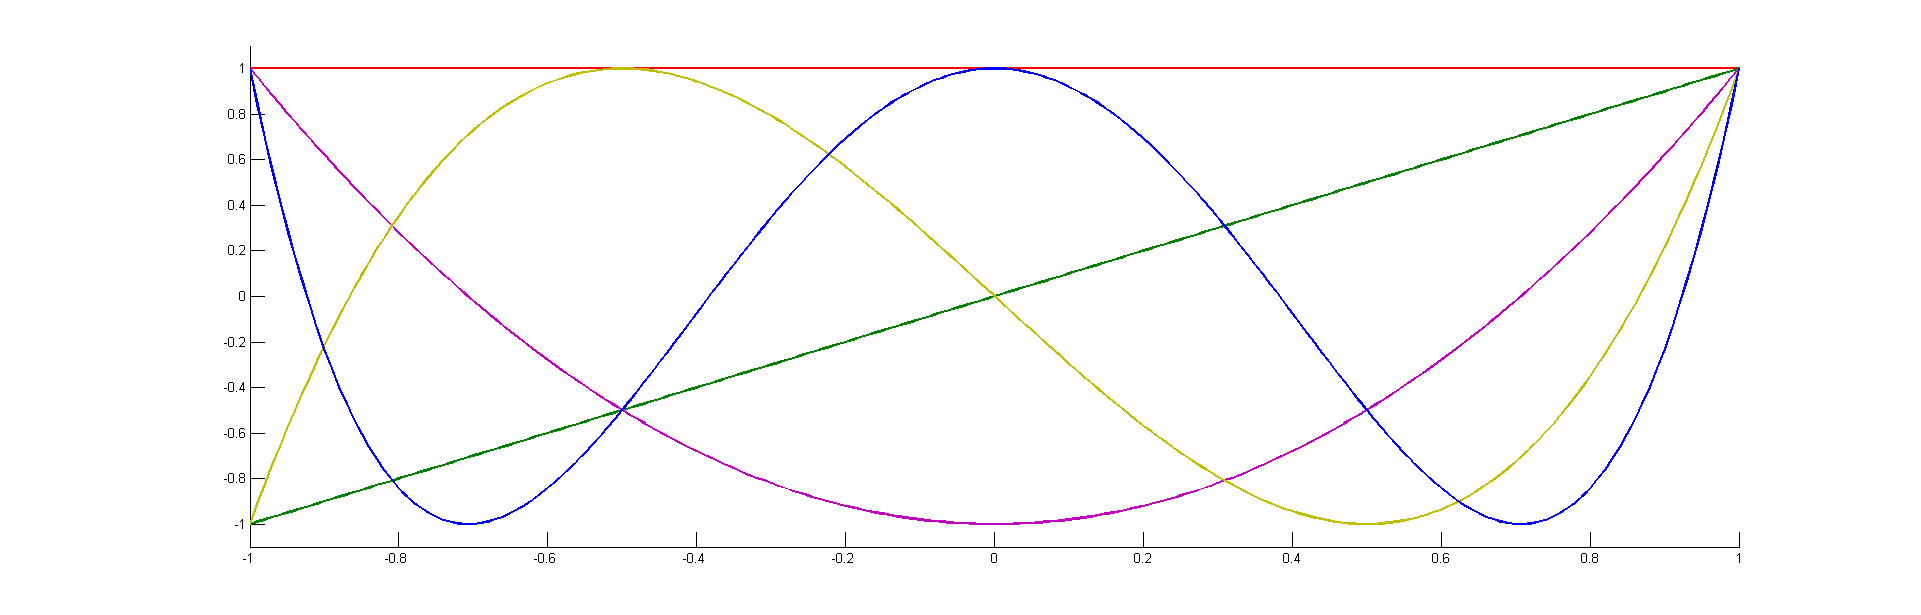
\includegraphics[width=\textwidth]{chebychev.png}
	\caption{Evaluatie van eerste tien Cheybchev veeltermen op 200 punten in [-1,1]}
	\label{chebychev}
\end{figure}

\section{Berekenen van interpolerende veelterm}
Zie bijlage \texttt{interpolate.m}\\
Dit algoritme berekent een interpolerende veelterm door de waarden $f(x)$ en evalueert die veelterm in de punten gegeven in $t$. Als we dit toepassen op respectievelijk $\cos(x)$ en $\frac{1}{1+6x^2}$ krijgen we grafiek \ref{interpolcos} en \ref{interpolexp}. We zien op het eerste zicht niet duidelijk verschil tussen het gebruik van equidistante interpolatiepunten en de nulpunten van de Chebychev-veelterm $T_n$.\\
\begin{figure}[htb]
\begin{subfigure}{0.5\textwidth}
\centering
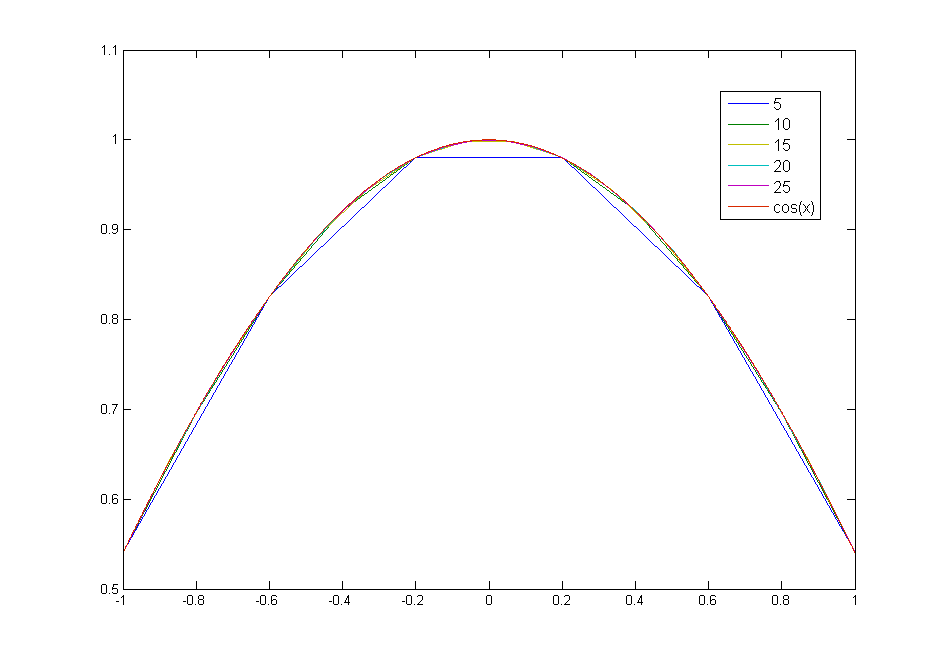
\includegraphics[width=\textwidth]{cosEqui.png}
\subcaption{Equidistant}
\end{subfigure}
\begin{subfigure}{0.5\textwidth}
\centering
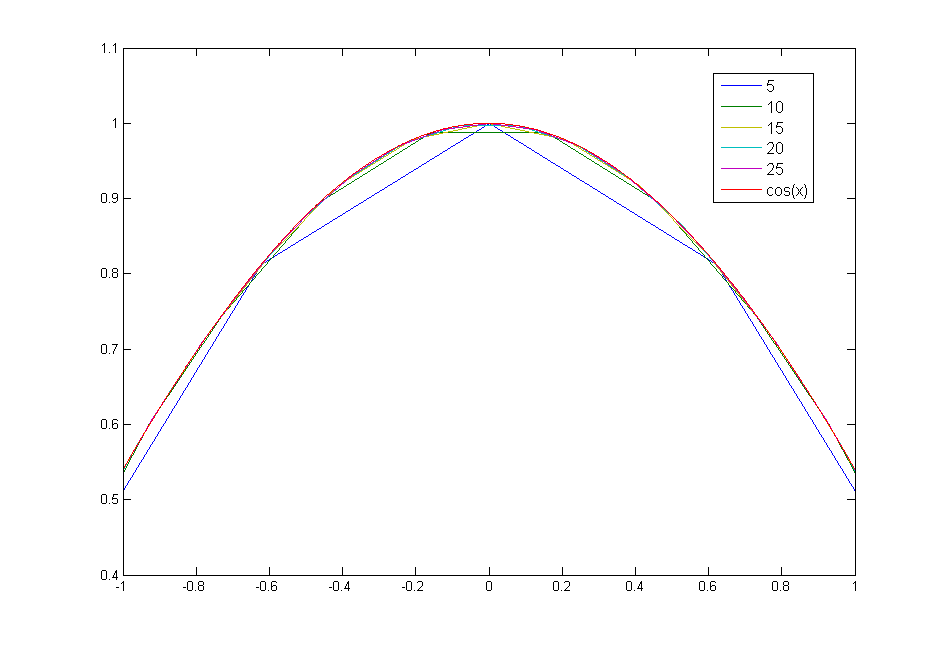
\includegraphics[width=\textwidth]{cosCheb.png}
\subcaption{Nulpunten van $T_n$}
\end{subfigure}

\caption{Enkele interpolerende veeltermen van $\cos(x)$}
\label{interpolcos}
\end{figure}

\begin{figure}[htb]
\begin{subfigure}{0.5\textwidth}
\centering
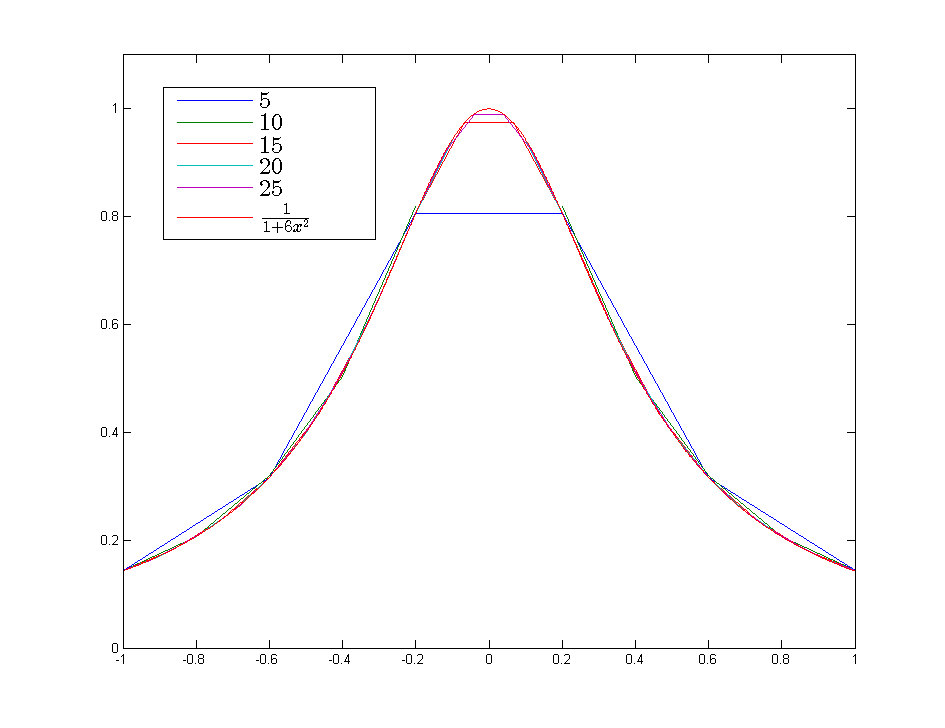
\includegraphics[width=\textwidth]{expEqui.png}
\subcaption{Equidistant}
\end{subfigure}
\begin{subfigure}{0.5\textwidth}
\centering
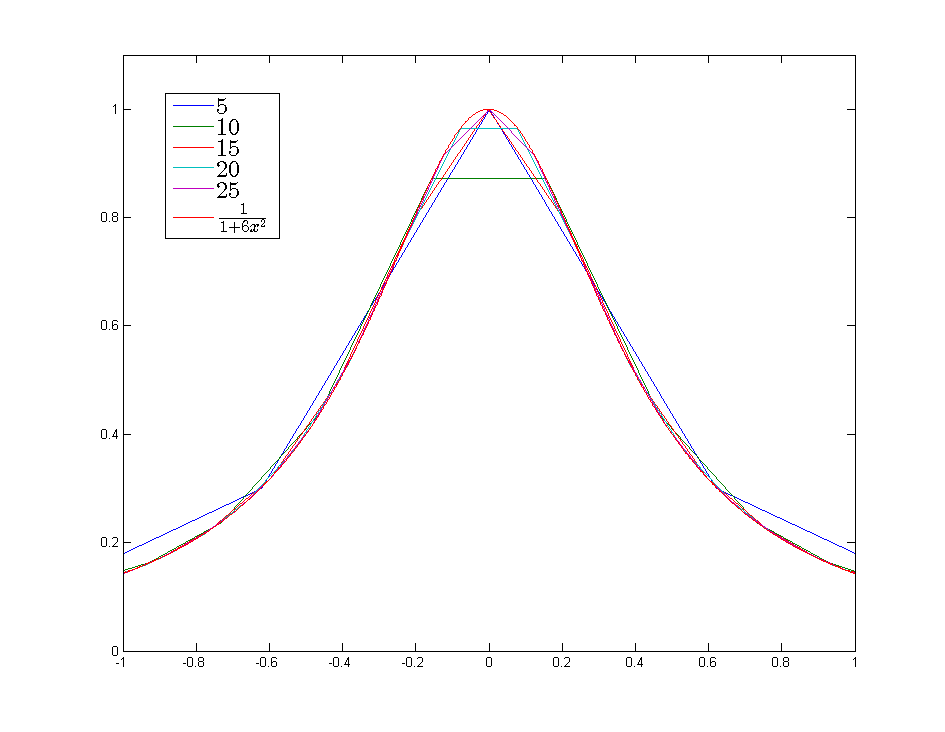
\includegraphics[width=\textwidth]{expCheb.png}
\subcaption{Nulpunten van $T_n$}
\end{subfigure}

\caption{Enkele interpolerende veeltermen van $\frac{1}{1+6x^2}$}
\label{interpolexp}
\end{figure}
 Bij een verdere analyse van de interpolatiefout blijkt echter dat de nulpunten van de Chebychev veeltermen een veel beter gespreide fout geven, de fout is ongeveer overal even groot. Voor illustratie, zie figuur \ref{errpol}. Bij de equidistante punten is er aan de rand van het interval een veel grotere fout aanwezig. Bij benaderingen van lagere graad is de absolute fout wel kleiner bij de equidistante punten. Het verschil aan de rand van het interpolatie-interval wordt veroorzaakt door de locatie van de interpolatiepunten. Als de nulpunten van $T_n$ worden gebruikt, liggen die veel meer geconcentreerd aan de rand van het interval, waardoor de fout aan de rand ongeveer even groot wordt als in het midden van het interval. Dit zorgt voor een fout die gemiddeld hoger is, maar minder hoge pieken heeft dan bij equidistante interpolatiepunten.\\
 \begin{figure}
 \begin{subfigure}{0.5\textwidth}
 \centering
 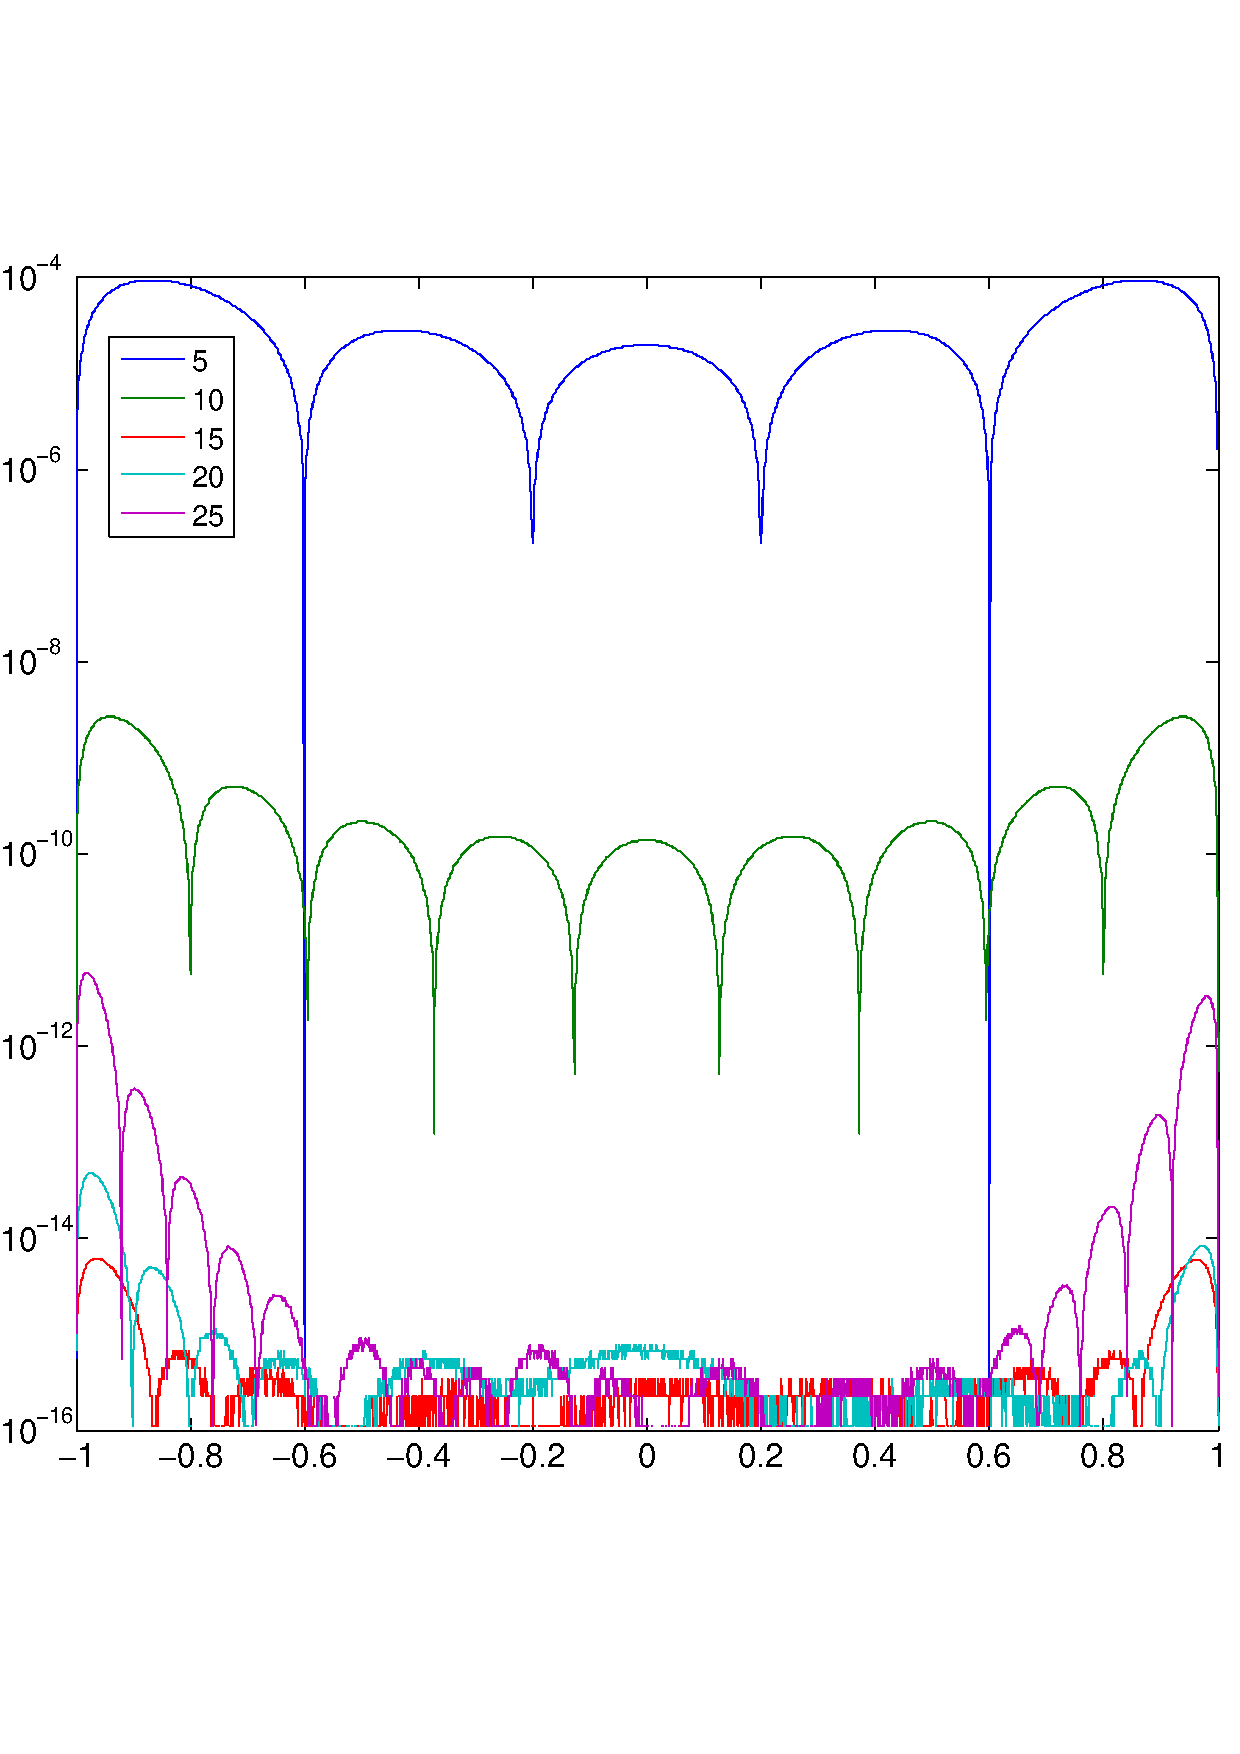
\includegraphics[width=\textwidth]{errorCos1.pdf}
 \subcaption{Equidistant, $\cos(x)$}
 \end{subfigure}
 \begin{subfigure}{0.5\textwidth}
 \centering
 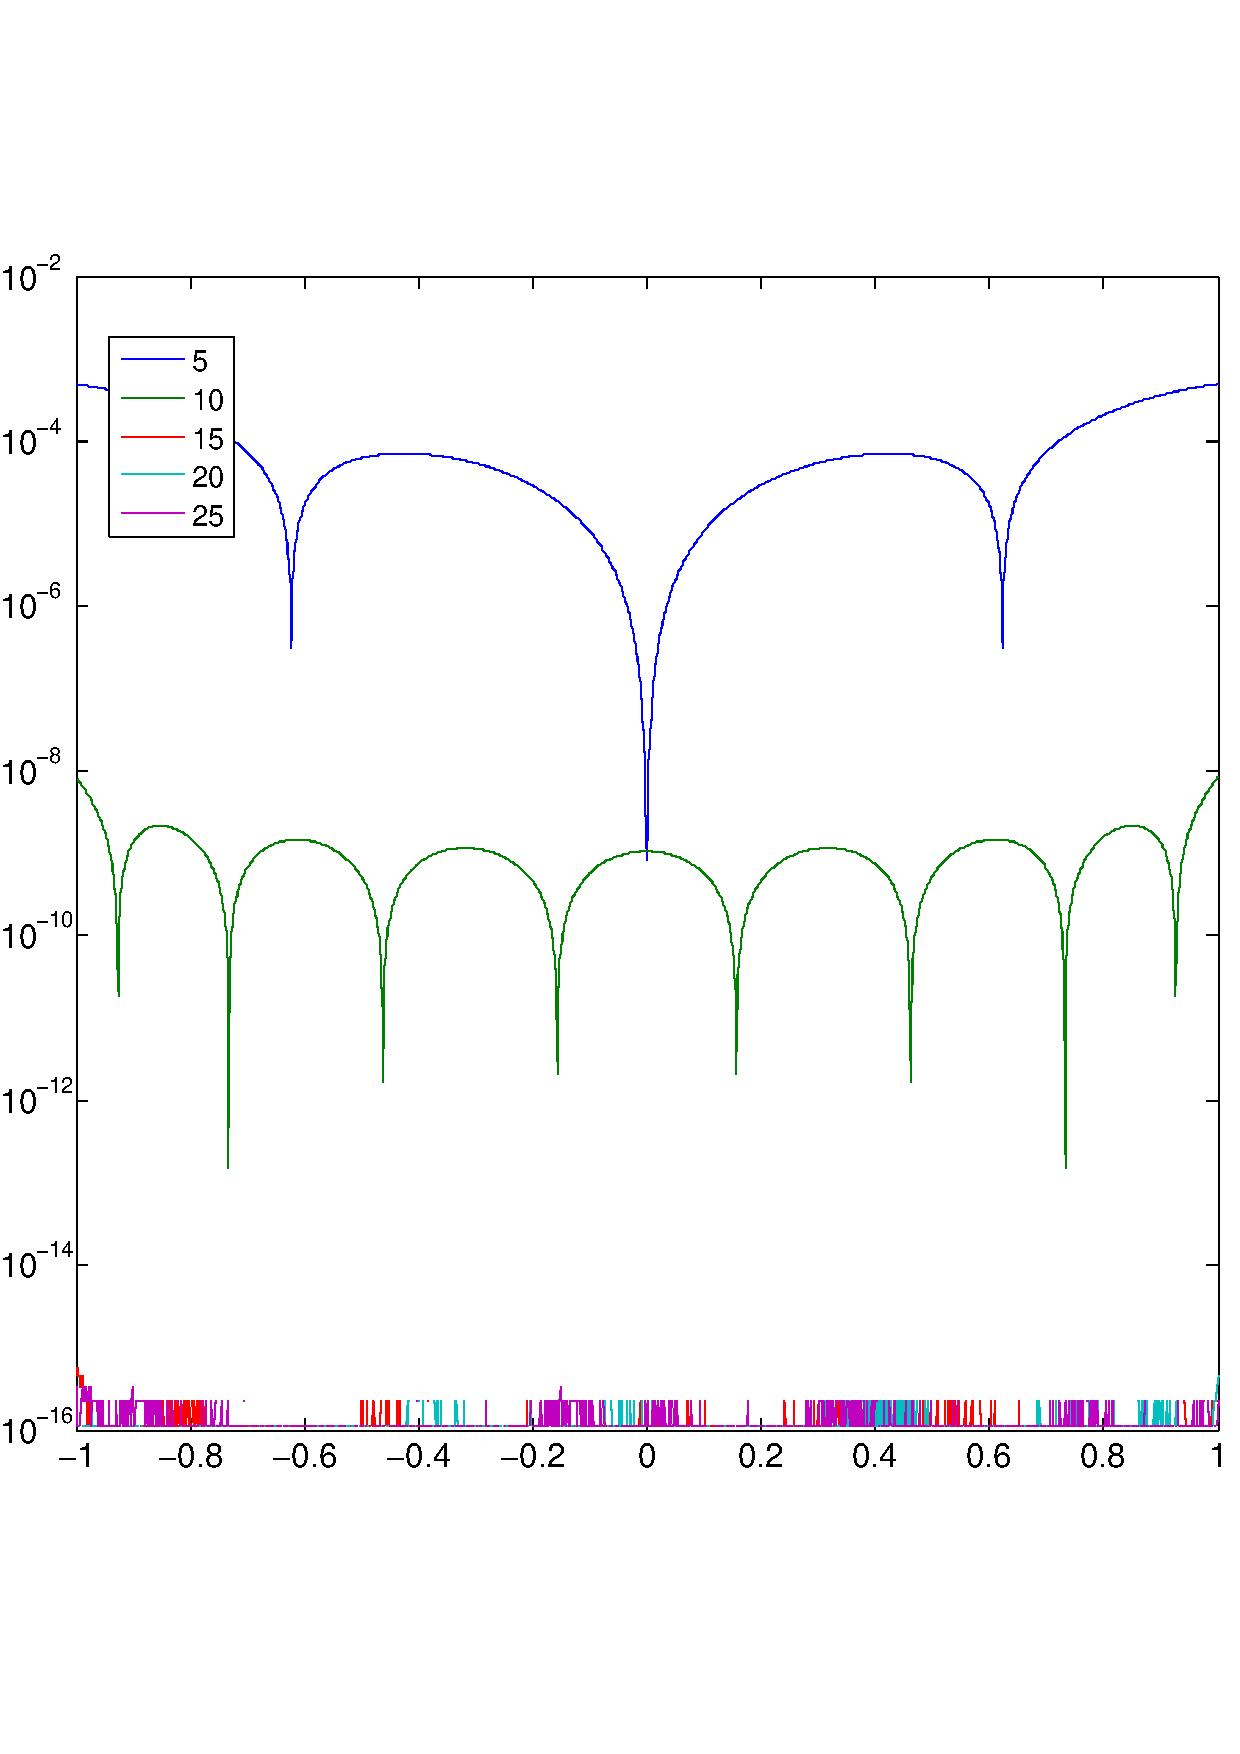
\includegraphics[width=\textwidth]{errorCos2.pdf}
 \subcaption{Nulpunten van $T_n$, $\cos(x)$}
 \end{subfigure}
 

 \begin{subfigure}{0.5\textwidth}
 \centering
 \includegraphics[width=\textwidth]{errorExp1.png}
 \subcaption{Equidistant, $\frac{1}{1+6x^2}$}
 \end{subfigure}
 \begin{subfigure}{0.5\textwidth}
 \centering
 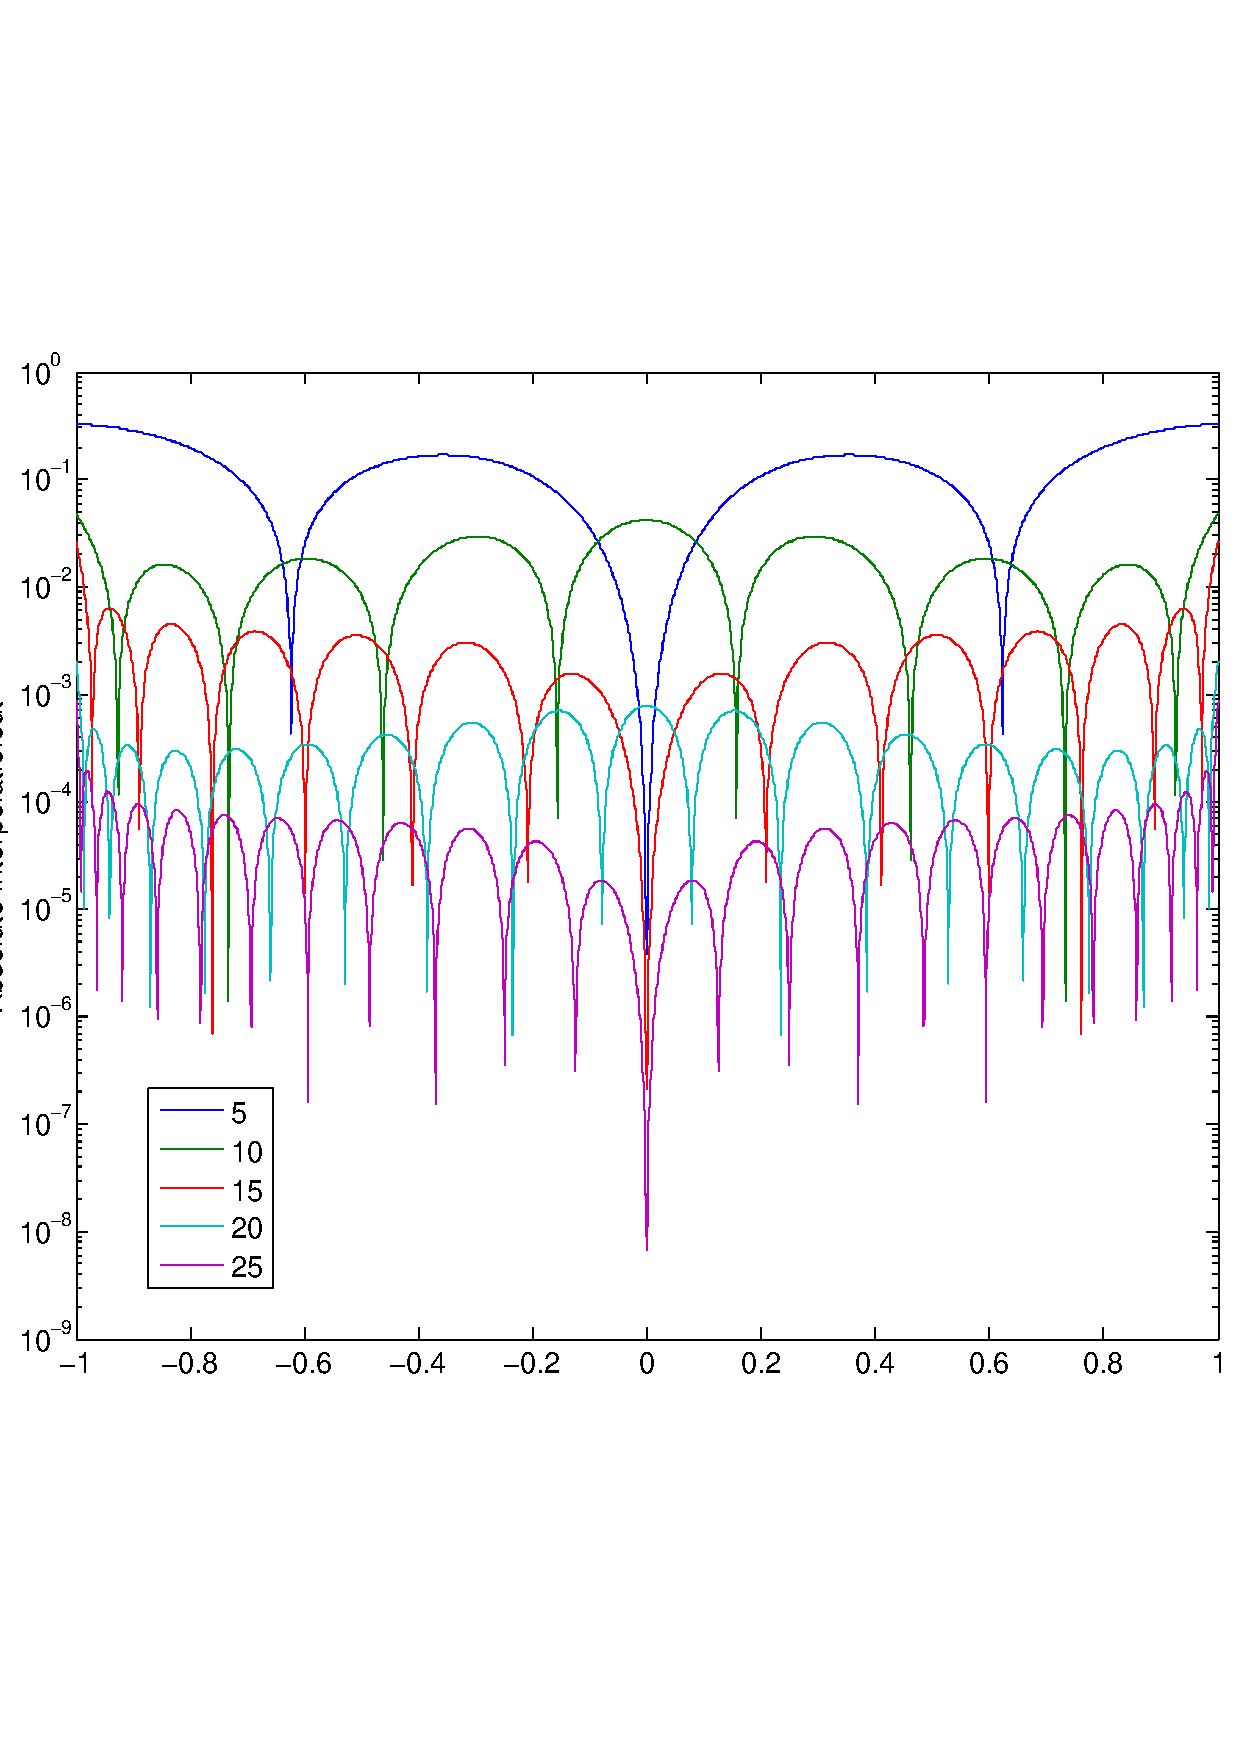
\includegraphics[width=\textwidth]{errorExp2.pdf}
 \subcaption{Nulpunten van $T_n$, $\frac{1}{1+6x^2}$}
 \end{subfigure}
 
 \caption{Absolute fout bij het interpoleren}
 \label{errpol}
 \end{figure}
 
 Als we de maximale fout in functie van de graad van de benadering uitzetten zien we ook dat bij hogere graad de equidistante punten weer onderdoen. We merken zelfs een stijging in de maximale fout vanaf een bepaalde punt. De Chebychev interpolatie daarentegen daalt in het begin ongeveer even snel, maar blijft bij hogere graad constant rond $\epsilon_{mach}$. Dit wordt duidelijk op figuur \ref{maxerr}. De stijgende \'staart\' van de grafiek voor equidistante punten wordt veroorzaakt door de zeer slechte benadering aan de rand van het interval. \\
 
 \begin{figure}
 \begin{subfigure}{0.5\textwidth}
 \centering
 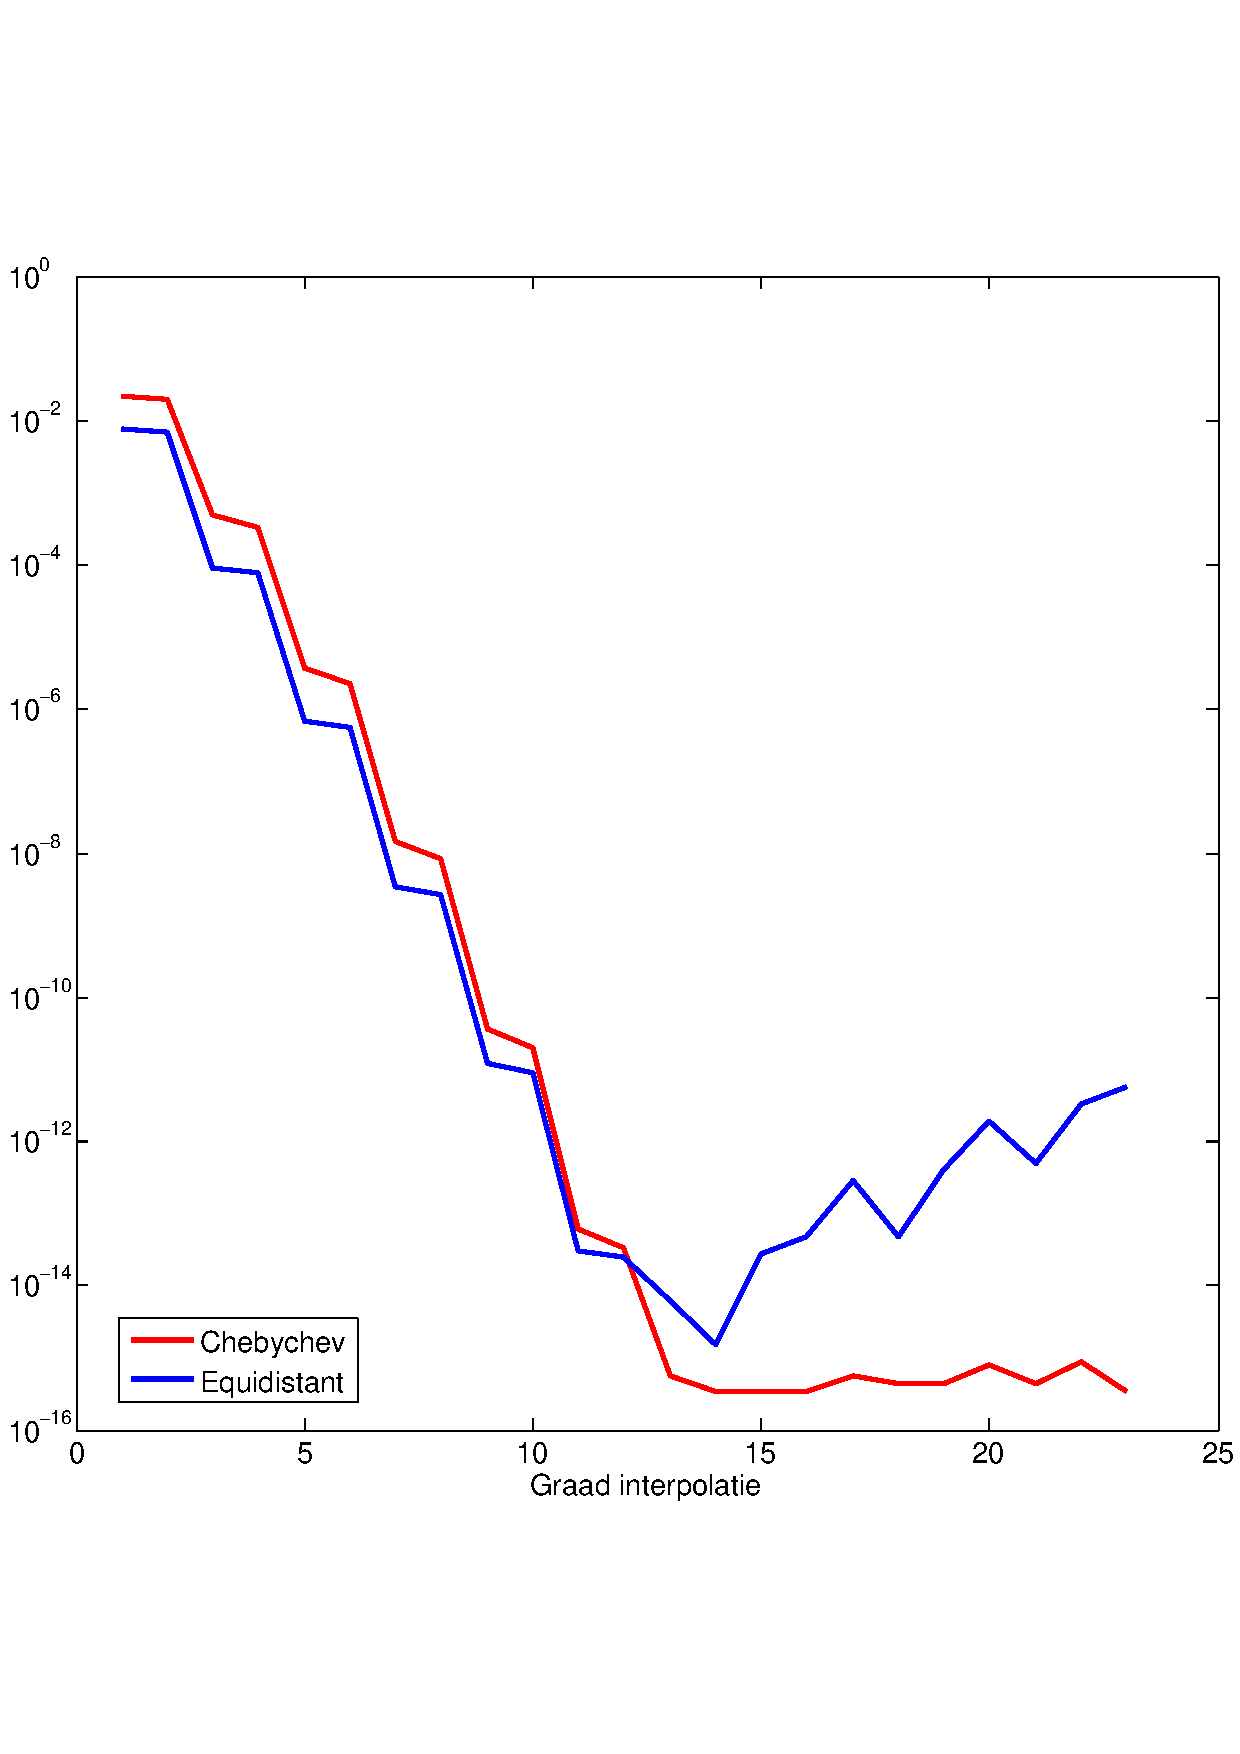
\includegraphics[width=0.9\textwidth]{maxCos.pdf}
 \subcaption{$\cos{x}$}
 \end{subfigure}
 \begin{subfigure}{0.5\textwidth}
 \centering
 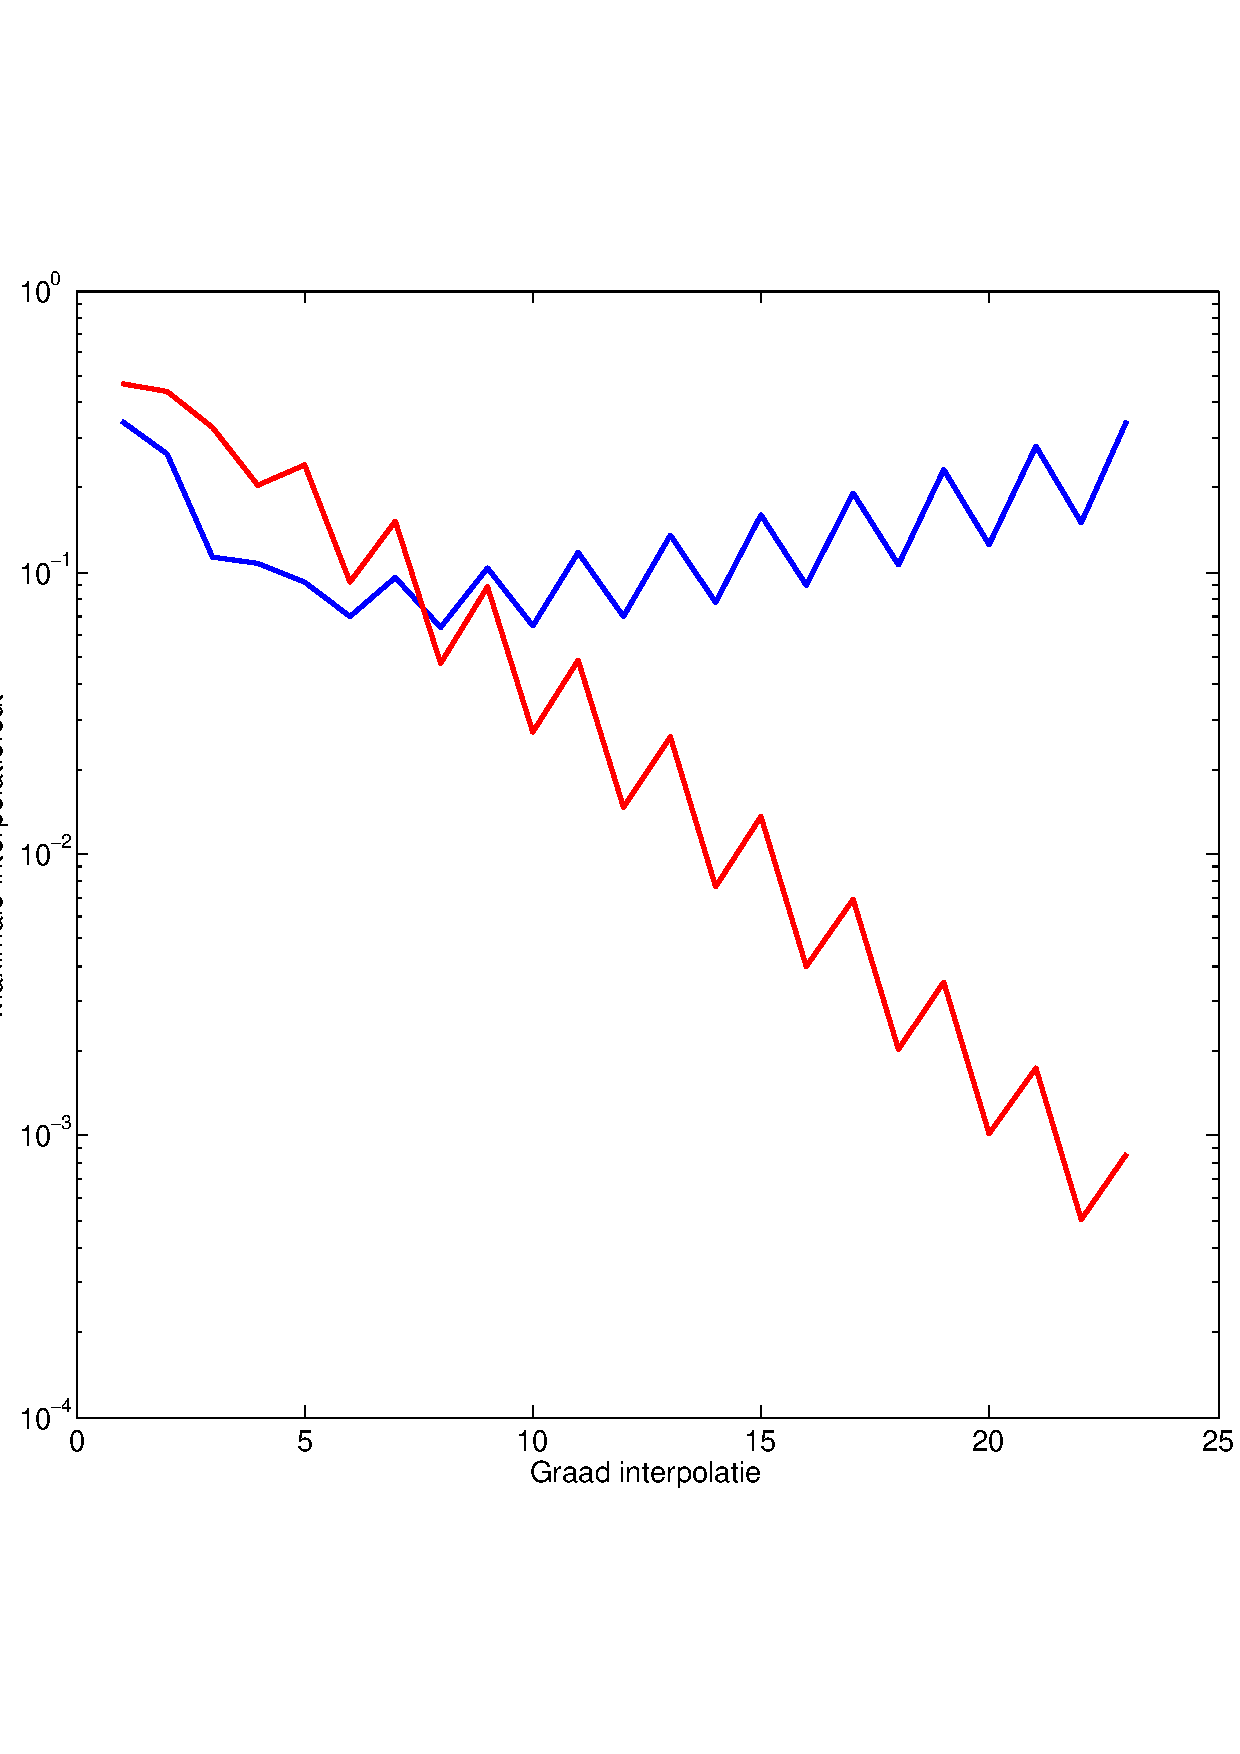
\includegraphics[width=0.9\textwidth]{maxExp.pdf}
 \subcaption{$\frac{1}{1+6x^2}$}
 \end{subfigure}
 
 \caption{Maximale interpolatiefout}
 \label{maxerr}
 \end{figure}
 
 Tot slot bestuderen we het conditiegetal van de matrix $M$ die gebruikt wordt in \texttt{eval\_recursion.m}. Als we dit voor beide methodes (equidistant en Chebychev) tonen in functie van de graad van benadering, zien we dat $k(M)$ exponenti\"eel stijgt voor beide methodes, maar minder snel bij equidistante interpolatiepunten. Bij een interpolatie van graad 25 is $k$ al van grootte-orde $10^7$ voor interpolatie in de nulpunten van $T_n$. Dit wil zeggen dat de interpolerende curve zelfs bij benaderingen van relatief lage graad al zeer gevoelig is aan kleine afwijkingen op de opgemeten waarden van $f(x)$. De toename van het conditiegetal wordt ge\"illustreerd in figuur \ref{condition}.
 
 \begin{center}
 \begin{figure}[!hb]
 \centering
  	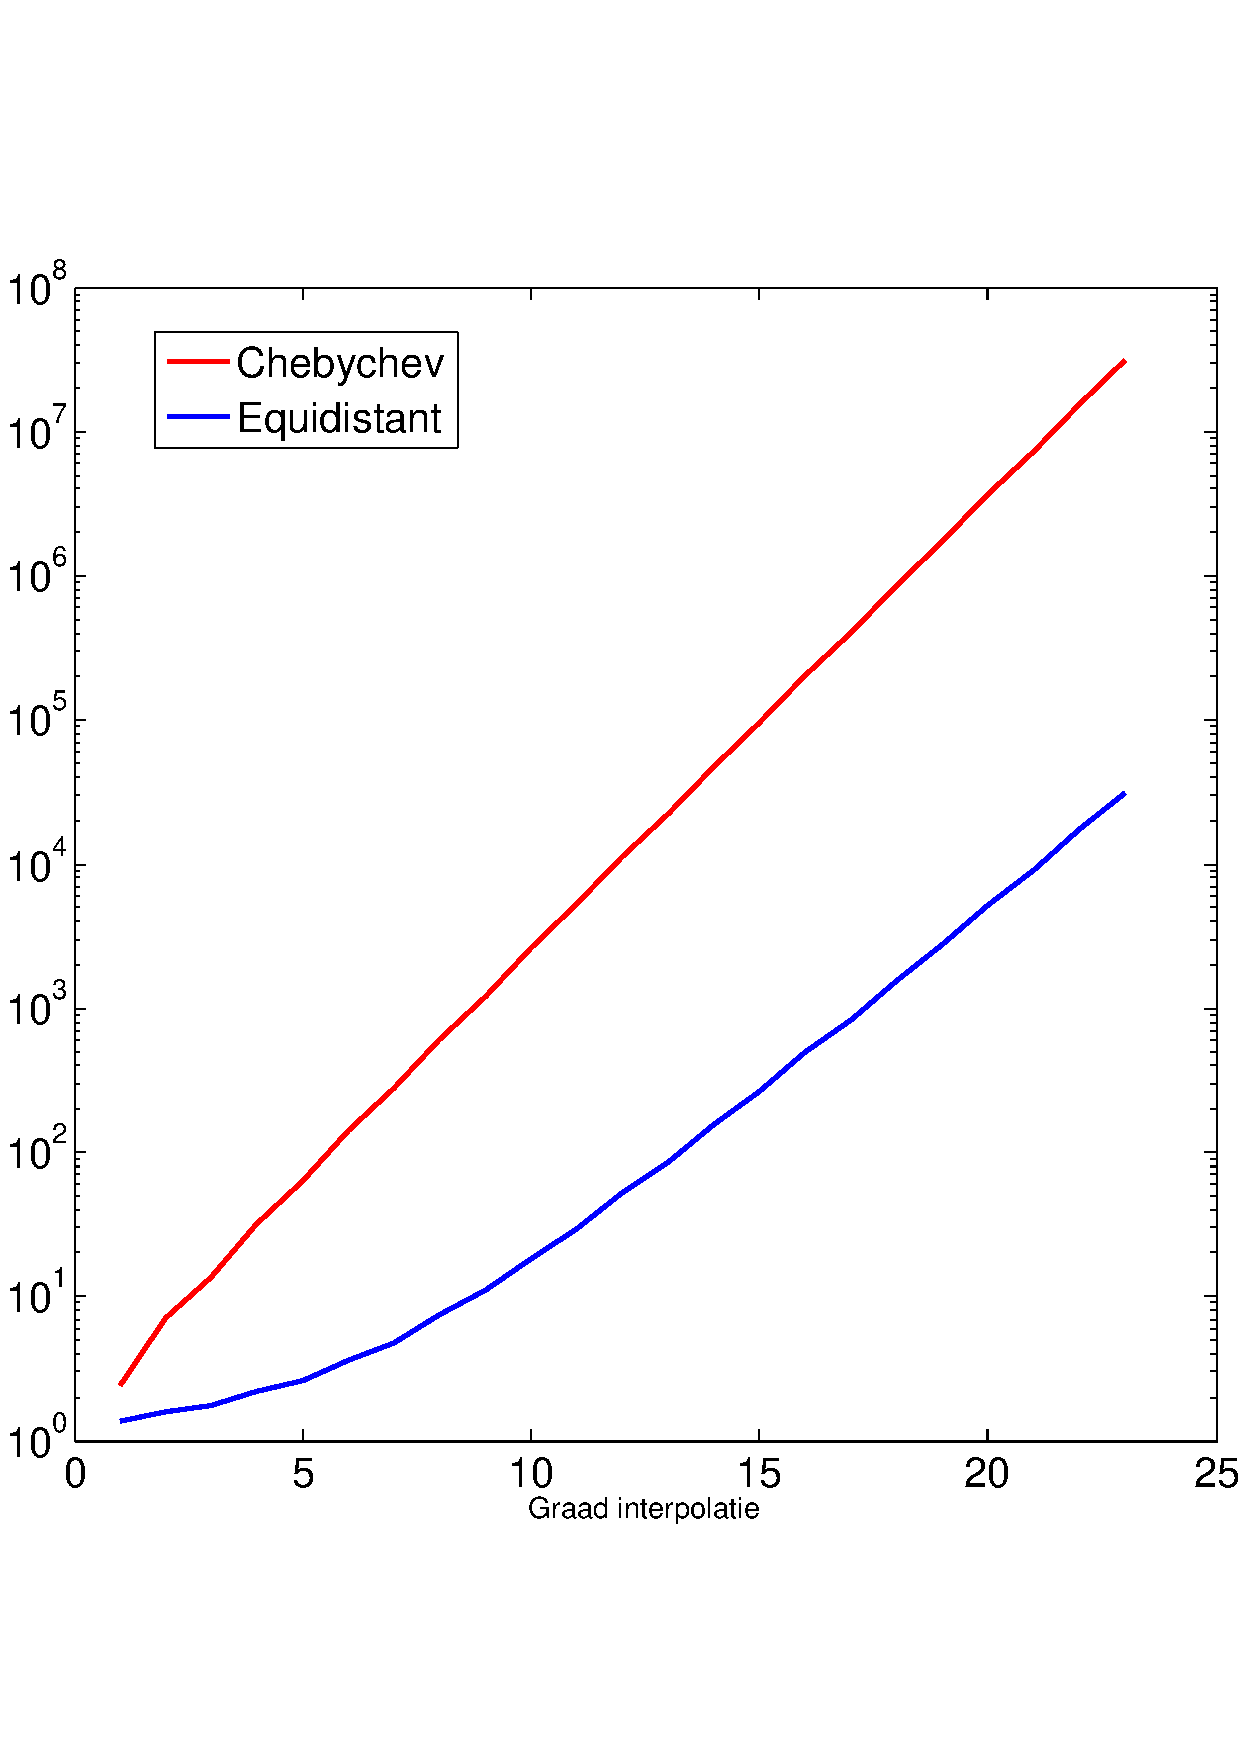
\includegraphics[width=0.4\textwidth]{condition.pdf}
  	\caption{Conditiegetal van M}
  	\label{condition}
  \end{figure}
 \end{center}
 
\section{Benaderen met trigonometrische veeltermen}
\subsection{function y = periotrig(x,K,M)}
todo code plakken
\subsection{Invloed van de parameter K op de benadering.}
Als te benaderende functie nemen we e^(-x^4). Deze functie wordt benaderd door trigoniometrische functies. De K-waarde geeft de indexwaarde van de laatste Xk-coefficient die behouden wordt opgegeven. Hoe lager de K-waarde, hoe minder termen er in de benadering aanwezig zijn. Een hogere K-waarde zal dus een betere benadering opleveren. Dit is ook te zien op de figuren. De eerste figuur toont de functie en de verschillende benaderingen. De tweede figuur geeft de norm van de fout weer van elke benadering. Hier is ook te zien dat bij een K-waarde van 64 de norm van de fout schommelt rond 10^-16. De fout ligt dus heel dicht bij de machinenauwkeurigheid.

\subsection{Benaderen van een gesloten kromme}
De click-functie geeft als output 2 vectoren. Een vector met X-waarden en een vector met Y-waarden. Deze 2 vectoren kunnen gebruikt worden als input van de periotrig functie.
todo figuur volgt nog wel ;)

 
 
\end{document}